\documentclass[boxes]{homework}

% This is a slightly-more-than-minimal document that uses the homework class.
% See the README at http://git.io/vZWL0 for complete documentation.

\name{傅申 PB20000051}        % Replace (Your Name) with your name.
\term{2022 秋}     % Replace (Current Term) with the current term.
\course{算法基础}    % Replace (Course Name) with the course name.
\hwnum{12}          % Replace (Number) with the number of the homework.
\hwname{作业}
\problemname{}
\solutionname{解:}

% Load any other packages you need here.
\usepackage[
    a4paper,
    top = 2.54cm,
    bottom = 2.54cm,
    left = 1.91cm,
    right = 1.91cm,
    includeheadfoot
]{geometry}
\fancyfootoffset{0pt} % make fancyhdr work properly
\usepackage{ctex}
\usepackage{tikz}
\usetikzlibrary{shapes}
\tikzset{
    >=latex,
    every node/.style={circle, draw, minimum size=1em, inner sep=.2em, align=center},
}

\begin{document}
%%%% Problem 22.3-6 %%%%
\problemchap{22}
\problempart{3}
\problemnumber{6}
\begin{problem}
证明: 在无向图中, 根据深度优先搜索算法是先探索 $(u, v)$ 还是先探索 $(v, u)$ 来将
边 $(u, v)$ 分类为树边或者后向边, 与根据分类列表中的 4 种类型的次序进行分类是等
价的.
\end{problem}
\begin{solution}
    由定理 22.10 可知, 无向图中的边要么是树边, 要么是后向边. 不妨假设此时在探索
    $(u, v)$, 若 $v$ 在此时被发现, 则 $(u, v)$ 先被探索, 且是树边; 若 $v$ 在此
    之前就被发现, 则 $(v, u)$ 在访问 $v$ 时就被探索了, 即 $(v, u)$ 先被探索, 且
    $(u, v)$ 是后向边. 因此可以根据 $(u, v)$ 的探索顺序将其分类为树边或者后向边.
\end{solution}

%%%% Problem 22.3-8 %%%%
\problemnumber{8}
\begin{problem}
请给出如下猜想的一个反例: 如果有向图 $G$ 包含一条从结点 $u$ 到结点 $v$ 的路径,
并且在对 $G$ 进行深度优先搜索时有 $u.d < v.d$, 则结点 $v$ 是结点 $u$ 在深度优先
森林中的一个后代.
\end{problem}
\begin{solution}
    如下, 探索顺序为 $w \to u \to v$, 且存在从 $u$ 到 $v$ 的路径 $u\to w \to v$,
    但是在深度优先森林中 $u$ 和 $v$ 互为兄弟结点.
    \begin{center}
        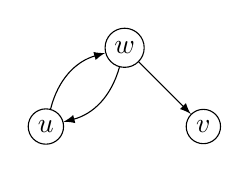
\begin{tikzpicture}
            \node (w) at (1, 1) {$w$};
            \node (u) at (0, 0) {$u$};
            \node (v) at (2, 0) {$v$};

            \path[->]
            (w) edge[bend left] (u)
            (u) edge[bend left] (w)
            (w) edge (v)
            ;
        \end{tikzpicture}
    \end{center}
\end{solution}

%%%% Problem 22.4-3 %%%%
\problempart{4}
\problemnumber{3}
\begin{problem}
给出一个算法来判断给定无向图 $G = (V, E)$ 是否包含一个环路. 算法运行时间应该在
$O(|V|)$ 量级, 且与 $|E|$ 无关.
\end{problem}
\begin{solution}
    考虑使用 DFS 来判断是否存在环路, 不过在 DFS 的过程中, 若当前结点 $u$ 探索边
    $(u, v)$ 时, $v$ 已经被发现且 $v$ 不是上一个访问的结点, 则说明存在环路, 停止
    搜索. 若 DFS 没有提前停止搜索, 则说明不存在环路.

    由于对于没有环路的无向图, $|E| \leqslant |V| - 1$, 因此, 若 DFS 提前结束, 则
    访问过的结点集合 $V_{v}$ 满足 $|V_{v}| \leqslant |V|$, 且搜索过的边集合
    $E_{v}$ 满足 $|E_{v}| \leqslant |V_{v}| - 1 + 1 = |V_{v}|$, 复杂度为
    $O(|V_{v}| + |E_{v}|) = O(|V|)$; 若 DFS 没有提前结束, 则
    $|E| \leqslant |V| - 1$, 复杂度为 $O(|V| + |E|) = O(|V|)$.
\end{solution}

%%%% Problem 22.5-3 %%%%
\problempart{5}
\problemnumber{3}
\begin{problem}
Bacon 教授声称, 如果在第二次深度优先搜索时使用原始图 $G$ 而不是图 $G$ 的转置图
$G^{\mathrm{T}}$, 并且以完成时间的递增次序来扫描结点, 则计算强连通分量的算法将会
更加简单. 这个更加简单的算法总是能计算出正确的结果吗?
\end{problem}
\begin{solution}
    不能, 考虑如下有向图, 它有两个强连通分量: $\{w, u\}$ 和 $\{v\}$.
    \begin{center}
        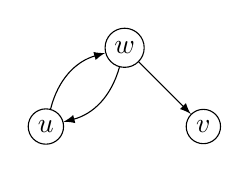
\begin{tikzpicture}
            \node (w) at (1, 1) {$w$};
            \node (u) at (0, 0) {$u$};
            \node (v) at (2, 0) {$v$};

            \path[->]
            (w) edge[bend left] (u)
            (u) edge[bend left] (w)
            (w) edge (v)
            ;
        \end{tikzpicture}
    \end{center}
    若第一次 DFS 从 $w$ 开始, 并先访问边 $(w, u)$, 则结果为
    \begin{center}
        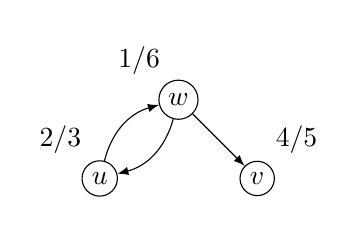
\begin{tikzpicture}
            \node (w) at (1, 1) {$w$};
            \node (u) at (0, 0) {$u$};
            \node (v) at (2, 0) {$v$};

            \node[draw=none] at (0.5, 1.5)  {1/6};
            \node[draw=none] at (-0.5, 0.5) {2/3};
            \node[draw=none] at (2.5, 0.5)  {4/5};
            \path[->]
            (w) edge[bend left] (u)
            (u) edge[bend left] (w)
            (w) edge (v)
            ;
        \end{tikzpicture}
    \end{center}
    因为按照完成时间的递增次序来扫描结点, 因此第二次 DFS 会从结点 $u$ 开始, 但是
    存在路径 $u \to w \to v$, 因此 $u$ 和 $v$ 将划分到同一个强连通分量中, 与正确
    的结果不符.
\end{solution}

%%%% Problem 23.2-5 %%%%
\problemchap{23}
\problempart{2}
\problemnumber{5}
\begin{problem}
假定图中的边权重取值全部为整数, 且在范围 $1 \sim |V|$ 内. Prim 算法最快能多快?
如果边的权重取值范围在 1 到某个常数 $W$ 之间呢?
\end{problem}
\begin{solution}
    当边权重的取值范围为 $1 \sim |V|$ 或 $1 \sim W$ 时, Prim 算法能达到
    $O(|E|\lg\lg |V|)$ 或 $O(|E|\lg\lg W)$ 的时间复杂度. 只需要使用 van Emde
    Boas 树来实现最小优先队列, 它对于 {\sc Extract-Min} 操作和
    {\sc Decrease-Key} 的时间均为 $O(\lg\lg |V|)$ 或 $O(\lg\lg W)$, 因此总的时间
    复杂度为 $O((|E| + |V|)\lg\lg |V|) = O(|E|\lg\lg |V|)$ 或 $O(|E|\lg\lg W)$.

    P.S. 我尝试实现一个 $O(|E|)$ 时间复杂度的 Prim 算法但是失败了, 主要是不知道
    如何在 $O(1)$ 的时间内维护优先队列中的最小值.
\end{solution}

%%%% Problem 24.1-3 %%%%    
\problemchap{24}
\problempart{1}
\problemnumber{3}
\begin{problem}
给定 $G=(V, E)$ 是一带权重且没有权重为负值的环路的有向图, 对于所有结点 $v\in V$,
从源结点 $s$ 到结点 $v$ 之间的最短路径中, 包含边的条数的最大值为 $m$. (这里, 判
断最短路径的根据是权重, 不是边的条数.) 请对算法 BELLMAN-FORD 进行简单修改, 可以
让其在 $m + 1$ 遍松弛操作之后终止, 即使 $m$ 不是事先知道的一个数值.
\end{problem}
\begin{solution}
    由上界性质可知, 在第 $m$ 遍松弛操作结束后, 所有结点的 $d$ 值都不会再改变, 因
    此在第 $m + 1$ 遍松弛操作中也不会有 $d$ 值改变. 因此可以检测每遍松弛操作中是
    否有 $d$ 值改变, 如果没有则可以提前结束松弛操作.
\end{solution}

%%%% Problem 24.2-2 %%%%
\problempart{2}
\problemnumber{2}
\begin{problem}
假定将 {\sc DAG-Shorest-Paths} 的第 3 行改为:

\textbf{for} the first $|V| - 1$ vertices, taken in topologically sorted
order

证明: 该算法的正确性保持不变.
\end{problem}
\begin{solution}
    拓扑排序次序中最后一个结点一定没有出边, 因此原算法中对于最后一个结点, 第 4
    行的 \textbf{for} 循环不会执行, 可以直接不考虑该结点. 所以修改后的算法正确性
    保持不变.
\end{solution}

\end{document}
